\section{Object reachable space shaping}

The task we are looking to automate is placed in the context of human-robot collaborative object manipulation. Where the robot is controlled in a human-centred manner and its actions take in consideration the human capacity in real-time. The robot behaviour we are searching to enable would consist to
\begin{enumerate}
    \item facilitate human's movements and augment his manipulation capacity
    \item prevent collisions of the object and the environment
    \item guide the operator towards the task completion
\end{enumerate}

\subsection{Human object manipulation scenario}
\begin{figure}[htb!]
    \centering
    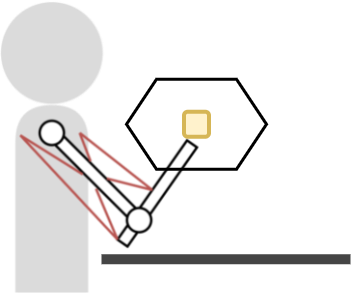
\includegraphics[width=0.3\textwidth]{Papers/lichie/g1.png}
    \caption{Manipulated object reachable space polytope of the human operator for initial scenario.}
    \label{fig:goal1}
\end{figure}


The human are applies forces onto the object he is manipulating, producing the objects motion
\begin{equation}
    m \ddot{\bm{x}} + \bm{g}= \bm{f}_h
\end{equation}
where $m$ is the mass of the object, and $\bm{g}$ is objects gravity. The human's force $\bm{f}_h$, as discussed in \ref{ch:force_poly_human}, is limited within the polytope $\mathcal{P}_{f,h}$
\begin{equation}
    \bm{f}_h \in \mathcal{P}_{f,h}
\end{equation}
The object's acceleration $\ddot{\bm{x}}$ can then be expressed as
\begin{equation}
    \ddot{\bm{x}} =  \frac{\bm{f}_h - \bm{g}}{m} = \frac{\bm{f}_h}{m}- \frac{\bm{g}}{m}
\end{equation}
As the human's force $\bm{f}_h$ is limited within a convex polytope, the set of all feasible accelerations $\ddot{\bm{x}}$ of the object can be expressed as a convex polytope $\mathcal{P}_a$ as well 
\begin{equation}
    \mathcal{P}_a = \{\ddot{\bm{x}} \in \mathbb{R}^m ~|~ m \ddot{\bm{x}} + \bm{g}= \bm{f}_h, \quad\bm{f}_h \in \mathcal{P}_{f,h} \}
\end{equation}


Give a certain object's state $\{\bm{x}_k,\dot{\bm{x}}_k\}$ and any human's force $\bm{f}_{h}$ applied on the object, producing an acceleration $\ddot{\bm{x}}_{h}$, the objects position in space $\bm{x}_{k+1}$ at the time $\Delta t$ can be found using the Euler backward integration
\begin{equation}
    \bm{x}_{k+1} = \bm{x}_{k} + \dot{\bm{x}}_{k}\Delta t  + \ddot{\bm{x}}\frac{\Delta t^2}{2} \\
    = \underbrace{\bm{x}_k + \dot{\bm{x}}_k\Delta t - \frac{\bm{g} \Delta t^2}{2m}}_{\text{constant}~~\bm{x}_{b,k}}+ \bm{f}_h\frac{\Delta t^2}{2m}
\end{equation}
The object's reachable space therefore depends directly on the human's force capacity and can be expressed as
\begin{equation}
    \mathcal{P}_x = \{\bm{x}_k \in \mathbb{R}^m ~|~ \bm{x}_k = \bm{x}_{b,k} + \bm{f}_h\frac{\Delta t^2}{2m}, \quad\bm{f}_h \in \mathcal{P}_{f,h} \}
\end{equation}
this scenario is illustrated on \Cref{fig:goal1}

% Human achievable force $\bm{F}_h$ and the robot achievable force $\bm{F}_r$ have a form of convex polytopes, the reachable set of object positions is a convex polytope as well. 

% \begin{equation}
%     \bm{x}_o(k) \in \mathcal{X}_o (k)
% \end{equation}

% The idea is to start from the object's reachable space or the set of all possible positions in space the object can attain based on its current position, velocity and the human capacity of force (or acceleration) generation. The reachable space has a form of convex polytope. The figure on the left, shows the scenario where the human operator is the only one handling the object. Then the reachable space will depend only on the human force capacity
% \begin{equation}
%     \bm{x}_o(k) = \bm{x}(k-1) + \dot{\bm{x}}_o(k-1)\Delta t +  \bm{F}_h(k)\frac{\Delta t^2}{2m_o}
% \end{equation}
% The reachable space (polytope) is shown in black in the \Cref{fig:goal1}.

\subsection{Human-robot initial collaboration}
\begin{figure}[htb!]
    \centering
    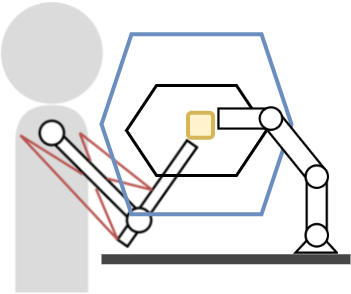
\includegraphics[width=0.3\textwidth]{Papers/lichie/g2.png}
    \caption{Operator's(black) and augmented(blue) object's reachable polytope for the second scenario.}
    \label{fig:goal2}
\end{figure}

In this scenario the operator and the robot apply forces on the object 
\begin{equation}
    m \ddot{\bm{x}} + \bm{g}= \bm{f}_h + \bm{f}_h
\end{equation}
As both human's and robot's forces are limited within their respective force capacity polytopes
\begin{equation}
    \bm{f}_h \in \mathcal{P}_{f,h}, \qquad  \bm{f}_r \in \mathcal{P}_{f,r}
\end{equation}
The object's overall acceleration capacity can be res presented as
\begin{equation}
    \mathcal{P}_a = \{\ddot{\bm{x}} \in \mathbb{R}^m ~|~ m \ddot{\bm{x}} + \bm{g}= \bm{f}_h +\bm{f}_r, ~\bm{f}_h \in \mathcal{P}_{f,h}, ~\bm{f}_r \in \mathcal{P}_{f,r} \}
\end{equation}

Then, the object's reachable space can be expressed as 
\begin{equation}
    \bm{x}_{k+1} = \underbrace{\bm{x}_k + \dot{\bm{x}}_k\Delta t - \frac{\bm{g} \Delta t^2}{2m}}_{\text{constant}~~\bm{x}_{b,k}}+ \bm{f}_h\frac{\Delta t^2}{2m}+ \bm{f}_r\frac{\Delta t^2}{2m}
\end{equation}
The object's reachable space therefore depends on both the human's and the robot's force capacity and can be expressed as
\begin{equation}
    \mathcal{P}_x = \{\bm{x}_k \in \mathbb{R}^m ~|~ \bm{x}_k = \bm{x}_{b,k} + \bm{f}_h\frac{\Delta t^2}{2m}+ \bm{f}_h\frac{\Delta t^2}{2m}, \quad\bm{f}_h \in \mathcal{P}_{f,h},~\bm{f}_r \in \mathcal{P}_{f,r} \}
\end{equation}
this scenario is illustrated on \Cref{fig:goal2}

\subsection{Human-robot collaboration with environment}
\begin{figure}[htb!]
    \centering
    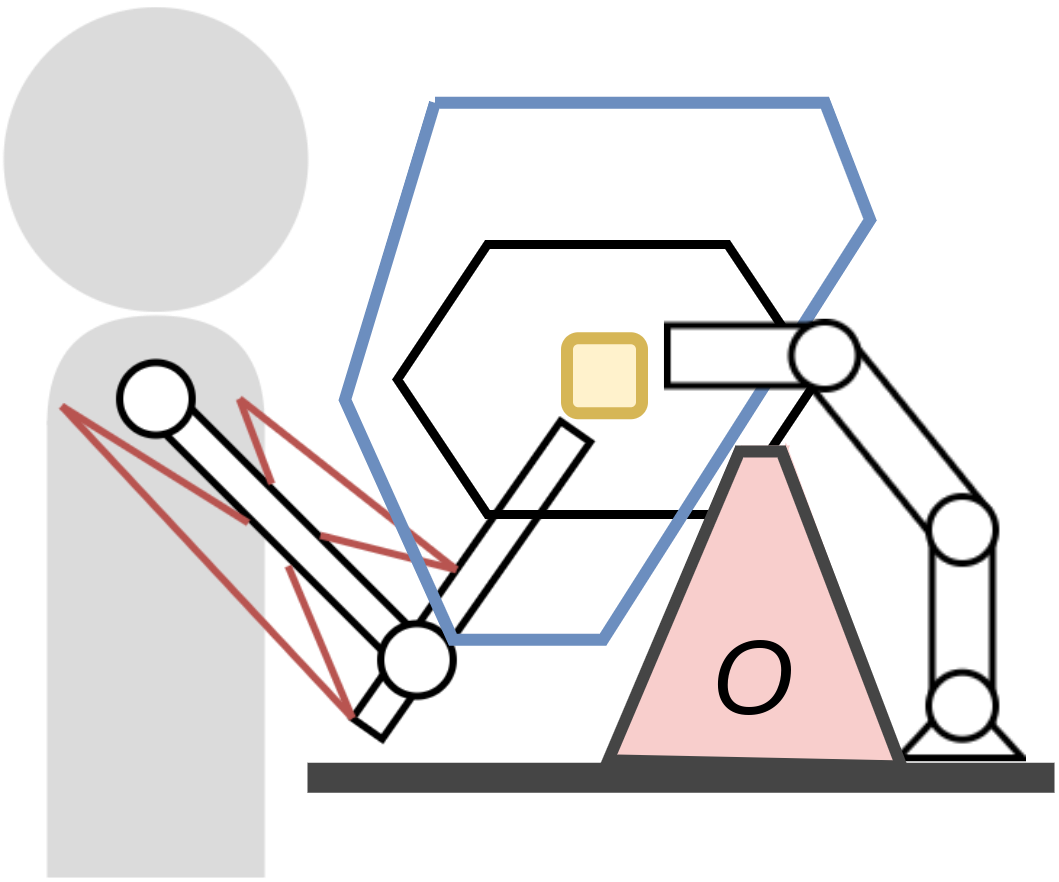
\includegraphics[width=0.3\textwidth]{Papers/lichie/g3.png}
    \caption{Operator's(black) and augmented(blue) reachable space polytope for the scenario with obstacles.}
    \label{fig:goal3}
\end{figure}
Third scenario, figure \ref{fig:goal3}, sows the extension of the second scenario. The difference is that the environment $\mathcal{O}$ is specified. Using the knowledge about the environment and the human force capacity $\mathcal{F}_h(k)$ the robot augments the reachable space on in the directions of the space which will not result in collision with the obstacles.

\begin{equation}
\begin{split}
    \bm{x}_o(k) =& \bm{x}(k-1) + \dot{\bm{x}}_o(k-1)\Delta t +  \left(\bm{F}_h(k)+\bm{F}_r(k)\right)\frac{\Delta t^2}{2m_o}\\ 
    \bm{F}_r\left(k\right) =& f\left(\bm{F}_r\left(k\right), \mathcal{F}_h\left(k\right), \mathcal{O}\right)
\end{split}
\end{equation}


\subsubsection*{TODOs}
\begin{itemize}
    \item Investigate ways of specifying the environment - simplified geometries: spheres, cubes, linear constraints, ...
    \item Develop ways to calculate distance and intersection of the reachable set and the environment. 
\end{itemize}

\subsection{Human-robot collaboration with environment and the task}
\begin{figure}[htb!]
    \centering
    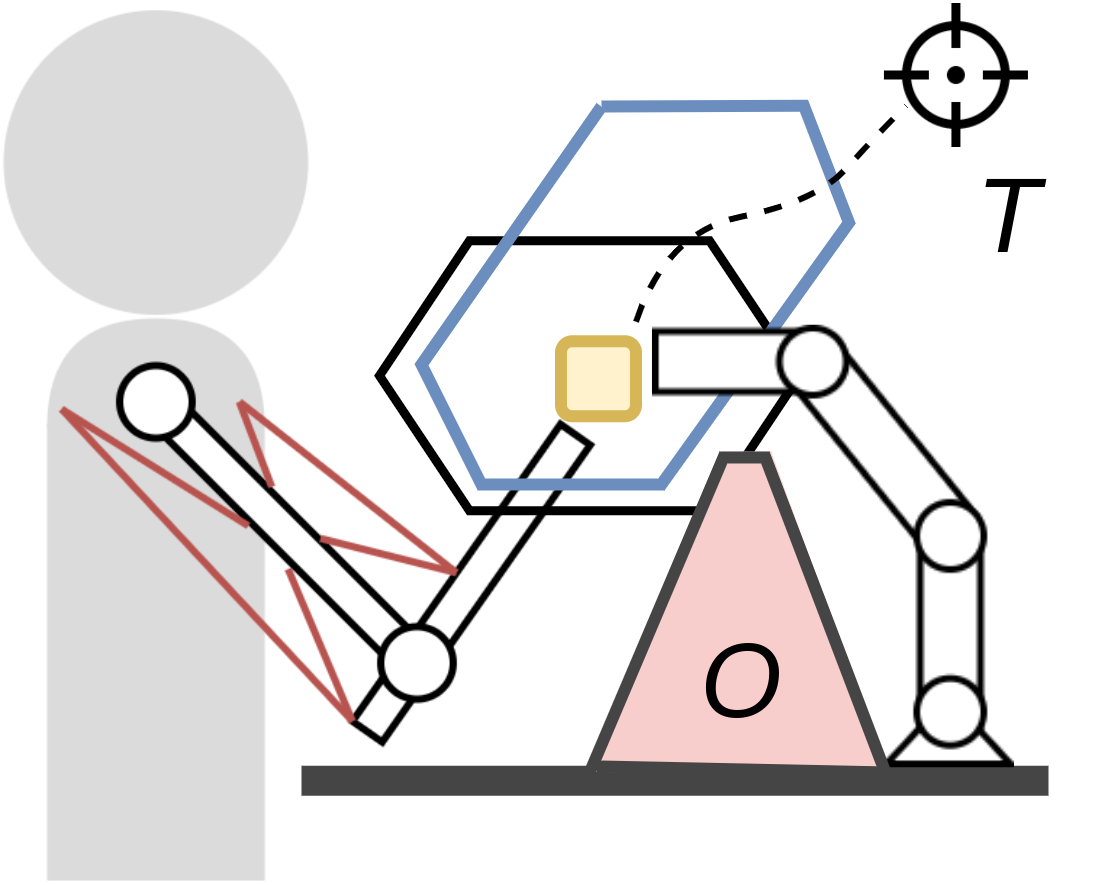
\includegraphics[width=0.3\textwidth]{Papers/lichie/g4.png}
    \caption{Operator's(black) and augmented(blue) reachable space polytope for the scenario with obstacles and the task defined.}
    \label{fig:goal4}
\end{figure}
Last scenario, figure \ref{fig:goal4}, the most complete scenario. In this scenario the environment $\mathcal{O}$ is specified as well as the knowledge about the task $\mathcal{T}$. Using the knowledge about the environment, the task and the human force capacity $\mathcal{F}_h(k)$ the robot augments the reachable space on in the directions of the space which will not result in collision with the obstacles.

\begin{equation}
\begin{split}
    \bm{x}_o(k) =& \bm{x}(k-1) + \dot{\bm{x}}_o(k-1)\Delta t +  \left(\bm{F}_h(k)+\bm{F}_r(k)\right)\frac{\Delta t^2}{2m_o}\\ 
    \bm{F}_r\left(k\right) =& f\left(\bm{F}_r\left(k\right), \mathcal{F}_h\left(k\right), \mathcal{O}, \mathacal{T}\right)
\end{split}
\end{equation}
